% !TeX program = xelatex
\documentclass[a4paper]{article}

\input{style/ch_xelatex.tex}
\input{style/scala.tex}

%代码段设置
\lstset{numbers=left,
	basicstyle=\tiny,
	numberstyle=\tiny,
	keywordstyle=\color{blue!70},
	commentstyle=\color{red!50!green!50!blue!50},
	frame=single, rulesepcolor=\color{red!20!green!20!blue!20},
	escapeinside=``
}

\graphicspath{ {images/} }
\usepackage{ctex}
\usepackage{graphicx}
\usepackage{color,framed}%文本框
\usepackage{listings}
\usepackage{caption}
\usepackage{amssymb}
\usepackage{enumerate}
\usepackage{xcolor}
\usepackage{bm} 
\usepackage{lastpage}%获得总页数
\usepackage{fancyhdr}
\usepackage{tabularx}  
\usepackage{geometry}
\usepackage{minted}
\usepackage{graphics}
\usepackage{subfigure}
\usepackage{float}
\usepackage{pdfpages}
\usepackage{pgfplots}
\pgfplotsset{width=10cm,compat=1.9}
\usepackage{multirow}
\usepackage{footnote}
\usepackage{booktabs}

%------------------------代码-------------------
\usepackage{xcolor} 
\usepackage{listings} 
\lstset{ 
	language=Verilog, % 设置默认语言为Verilog
	breaklines,%自动换行
	basicstyle=\small\ttfamily, % 使用等宽字体
	escapeinside=``,
	keywordstyle=\color{ blue!70} \bfseries,
	commentstyle=\color{red!50!green!50!blue!50},% 
	stringstyle=\ttfamily,% 
	extendedchars=false,% 
	linewidth=\textwidth,% 
	numbers=left,% 
	numberstyle=\tiny \color{blue!50},% 
	frame=trbl,% 
	rulesepcolor= \color{ red!20!green!20!blue!20} 
}

%-------------------------页面边距--------------
\geometry{a4paper,left=2.3cm,right=2.3cm,top=2.7cm,bottom=2.7cm}
%-------------------------页眉页脚--------------
\usepackage{fancyhdr}
\pagestyle{fancy}
\lhead{\kaishu \leftmark}
% \chead{}
\rhead{\kaishu 计算机体系结构实验报告}%加粗\bfseries 
\lfoot{}
\cfoot{\thepage}
\rfoot{}
\renewcommand{\headrulewidth}{0.1pt}  
\renewcommand{\footrulewidth}{0pt}%去掉横线
\newcommand{\HRule}{\rule{\linewidth}{0.5mm}}%标题横线
\newcommand{\HRulegrossa}{\rule{\linewidth}{1.2mm}}
\setlength{\textfloatsep}{10mm}%设置图片的前后间距
%--------------------文档内容--------------------

\begin{document}
	\renewcommand{\contentsname}{目\ 录}
	\renewcommand{\appendixname}{附录}
	\renewcommand{\appendixpagename}{附录}
	\renewcommand{\refname}{参考文献} 
	\renewcommand{\figurename}{图}
	\renewcommand{\tablename}{表}
	\renewcommand{\today}{\number\year 年 \number\month 月 \number\day 日}
	
	%-------------------------封面----------------
	\begin{titlepage}
		\begin{center}
			
\includegraphics[width=0.8\textwidth]{NKU.png}\\[1cm]
			\vspace{20mm}
				\textbf{\huge\textbf{\kaishu{计算机学院}}}\\[0.5cm]
				\textbf{\huge{\kaishu{计算机网络实验报告}}}\\[2.3cm]
				\textbf{\Huge\textbf{\kaishu{设计可靠传输协议并编程实现}}}
			
			\vspace{\fill}
			
			% \textbf{\Large \textbf{计算机网络实验报告}}\\[0.8cm]
			% \HRule \\[0.9cm]
			% \HRule \\[2.0cm]
			\centering
				\textsc{\LARGE \kaishu{姓名\ :\ 王一诺}}\\[0.5cm]
				\textsc{\LARGE \kaishu{学号\ :\ 2312331}}\\[0.5cm]
				\textsc{\LARGE \kaishu{专业\ :\ 计算机科学与技术}}\\[0.5cm]
			
			\vfill
			{\Large \today}
		\end{center}
	\end{titlepage}
	
	\renewcommand {\thefigure}{\thesection{}.\arabic{figure}}%图片按章标号
	\renewcommand{\figurename}{图}
	\renewcommand{\contentsname}{目录}  
	\cfoot{\thepage\ of \pageref{LastPage}}%当前页 of 总页数
	
	
	% 生成目录
	\clearpage
	\tableofcontents
	\newpage
	\setcounter{figure}{0} % 每章开始前重置图片计数器
	
	
	\section{实验要求与任务}
	\paragraph{实验要求：}
	利用数据报套接字在用户空间实现面向连接的可靠数据传输，功能包括：
	\begin{enumerate}
		\item 连接管理：包括建立连接、关闭连接和异常处理。
		\item 差错检测：使用校验和进行差错检测。
		\item 确认重传：支持流水线方式，采用选择确认。
		\item 流量控制：发送窗口和接收窗口使用相同的固定大小窗口。
		\item 拥塞控制：实现RENO算法。
	\end{enumerate}
	\paragraph{实验任务：}
	\begin{enumerate}
		\item 实现单向数据传输，控制信息需要实现双向交互。
		\item 给出详细的协议设计说明。
		\item 给出详细的实现方法说明。
		\item 利用C或C++语言，使用基本的Socket函数进行程序编写，不允许使用CSocket等封装后的类。
		\item 在规定的测试环境中，完成给定测试文件的传输，显示传输时间和平均吞吐率，并观察不同发送窗口和接收窗口大小对传输性能的影响，以及不同丢包率对传输性能的影响。
		\item 编写的程序应该结构清晰，具有较好的可读性。
	\end{enumerate}
	
	\section{协议设计说明}
	本实验旨在基于无连接的UDP协议，在应用层实现一套可靠的数据传输协议（Reliable UDP）。协议的设计参考了TCP的核心机制，并针对实验要求进行了简化与适配。协议报文格式设计紧凑，采用二进制流的方式进行封装，确保传输效率。
	
	\paragraph{报文头部设计：}
	为了支持序列号、确认应答、窗口通告及校验和等功能，定义了如下的报文头部结构（采用1字节对齐）：
	
	\begin{table}[H]
		\centering
		\begin{tabular}{|c|c|c|c|}
			\hline
			\multicolumn{2}{|c|}{32位 序列号 (seq)} & \multicolumn{2}{c|}{32位 确认号 (ack)} \\ \hline
			16位 数据长度 (len) & 16位 窗口大小 (wnd) & 16位 标志位 (flags) & 16位 校验和 (checksum) \\ \hline
			\multicolumn{4}{|c|}{32位 选择确认掩码 (sack)} \\ \hline
		\end{tabular}
		\caption{RUDP 协议报文头部结构}
	\end{table}
	
	\begin{itemize}
		\item \textbf{seq (Sequence Number)}：标识数据包的顺序，用于接收端重组数据及检测乱序。
		\item \textbf{ack (Acknowledgment Number)}：累计确认号，表示期望收到的下一个字节序列号。
		\item \textbf{flags}：控制位，用于标识包类型。本协议定义了如下标志：
		\begin{itemize}
			\item \texttt{FLAG\_SYN (0x0001)}: 用于建立连接。
			\item \texttt{FLAG\_ACK (0x0002)}: 确认应答。
			\item \texttt{FLAG\_FIN (0x0004)}: 用于断开连接。
			\item \texttt{FLAG\_META (0x0010)}: 用于传输文件元数据（文件名、大小）。
		\end{itemize}
		\item \textbf{wnd (Window)}：接收窗口大小，单位为分片数，用于流量控制。
		\item \textbf{sack (Selective ACK)}：32位掩码，用于告知发送端哪些非连续的数据块已收到，支持高效的重传。
		\item \textbf{checksum}：16位互联网校验和，覆盖头部和数据载荷。
	\end{itemize}
	
	\section{逐步具体实现}
	接下里从底层函数的设计开始，逐步介绍各个功能模块的实现并展示相关代码。
	
	\subsection{底层函数：套接字操作}
	本实验基于UDP协议实现可靠传输，因此首先需要构建跨平台的UDP套接字基础环境。由于Windows和Linux在Socket API上存在细微差异（如头文件包含、初始化过程及错误处理），我在代码中使用了宏定义 \_WIN32 来区分操作系统。在实现中，make\_udp\_socket 函数是核心，它负责创建一个数据报类型的套接字 SOCK\_DGRAM，并将其绑定到指定的本地IP地址和端口上。这是后续所有数据收发的基础。此外，resolve\_address 函数利用 inet\_pton 将字符串形式的IP地址转换为网络字节序的二进制结构，确保地址信息的正确性。

	\begin{lstlisting}[language=C++]
		// 跨平台初始化 Socket 库
		bool init_socket_lib() {
		#ifdef _WIN32
			static bool inited = false;
			if (inited) return true;
			WSADATA data;
			// 初始化 Winsock
			if (WSAStartup(MAKEWORD(2, 2), &data) != 0) {
				return false;
			}
			inited = true;
		#endif
			return true;
		}
		
		// 创建并绑定 UDP 套接字
		SOCKET make_udp_socket(const std::string& bind_ip, uint16_t bind_port) {
			// 创建 UDP 套接字 (AF_INET: IPv4, SOCK_DGRAM: 数据报)
			SOCKET s = socket(AF_INET, SOCK_DGRAM, 0);
			if (s == INVALID_SOCKET) return INVALID_SOCKET;
		
			sockaddr_in addr{};
			addr.sin_family = AF_INET;
			addr.sin_port = htons(bind_port); // 端口转为网络字节序
			if (bind_ip.empty()) {
				addr.sin_addr.s_addr = INADDR_ANY; // 监听所有网卡
			} else {
				// 将 IP 字符串转换为二进制地址
				if (inet_pton(AF_INET, bind_ip.c_str(), &addr.sin_addr) != 1) {
					close_socket(s);
					return INVALID_SOCKET;
				}
			}
			// 绑定套接字到指定地址
			if (bind(s, reinterpret_cast<sockaddr*>(&addr), sizeof(addr)) == SOCKET_ERROR) {
				close_socket(s);
				return INVALID_SOCKET;
			}
			return s;
		}
	\end{lstlisting}

	\begin{itemize}
		\item \texttt{环境初始化}: 在Windows环境下，使用Socket API前必须调用 WSAStartup 进行初始化，而Linux则不需要。代码通过 \#ifdef \_WIN32 实现了这一兼容性处理。
		\item \texttt{Socket创建}: socket(AF\_INET, SOCK\_DGRAM, 0) 用于创建一个IPv4的UDP套接字。AF\_INET 指定地址族为IPv4，SOCK\_DGRAM 指定为数据报服务，符合UDP无连接的特性。
		\item \texttt{地址转换与绑定}: bind 函数将套接字与特定的IP和端口关联。htons 函数将主机字节序的端口号转换为网络大端字节序。inet\_pton 是一个支持IPv4/IPv6的地址转换函数，用于将点分十进制IP字符串转换为 in\_addr 结构。如果 bind\_ip 为空，则使用 INADDR\_ANY，表示接收本机所有网卡的数据。
	\end{itemize}

	\subsection{数据包的定义与序列化}
	为了在无结构的UDP数据流之上实现可靠传输，必须定义严格的应用层协议报文格式。我设计了 PacketHeader 结构体，包含序列号、确认号、窗口大小、SACK掩码等关键字段。为了解决不同机器间内存对齐方式可能不一致的问题，使用了 \#pragma pack(push, 1) 指令强制结构体按1字节对齐。在发送数据前，需要将主机字节序 Host Byte Order 转换为网络字节序 Network Byte Order ，接收时则进行逆操作。serialize\_packet 函数负责将内存中的 Packet 对象打包成可以在网络上传输的字节流，并计算校验和。

	\begin{lstlisting}[language=C++]
		// 数据包头部，保持紧凑布局
		#pragma pack(push, 1)
		struct PacketHeader {
			uint32_t seq;       // 序列号
			uint32_t ack;       // 确认号
			uint16_t len;       // 载荷长度
			uint16_t wnd;       // 窗口大小
			uint16_t flags;     // 标志位 (SYN, ACK, FIN, META)
			uint32_t sack;      // 选择确认窗口
			uint16_t checksum;  // 校验和
		};
		#pragma pack(pop)

		// 序列化数据包
		std::vector<uint8_t> serialize_packet(const Packet& pkt) {
			PacketHeader hdr_net{};
			// 主机字节序 -> 网络字节序
			hdr_net.seq = htonl(pkt.header.seq);
			hdr_net.ack = htonl(pkt.header.ack);
			hdr_net.len = htons(pkt.header.len);
			hdr_net.wnd = htons(pkt.header.wnd);
			hdr_net.flags = htons(pkt.header.flags);
			hdr_net.sack = htonl(pkt.header.sack);
			hdr_net.checksum = 0; // 校验和计算前先置0

			// 拼接头部和数据载荷
			std::vector<uint8_t> buffer(sizeof(PacketHeader) + pkt.payload.size());
			std::memcpy(buffer.data(), &hdr_net, sizeof(PacketHeader));
			if (!pkt.payload.empty()) {
				std::memcpy(buffer.data() + sizeof(PacketHeader),
							pkt.payload.data(), pkt.payload.size());
			}
			// 计算校验和并回填
			uint16_t sum = checksum16(buffer.data(), buffer.size());
			reinterpret_cast<PacketHeader*>(buffer.data())->checksum = htons(sum);
			return buffer;
		}
	\end{lstlisting}

	\begin{itemize}
		\item \texttt{结构体对齐}: \#pragma pack(push, 1) 确保 PacketHeader 结构体中的字段在内存中是连续存放的，没有编译器自动填充的空隙。这对直接内存拷贝（memcpy）进行网络传输至关重要，保证了接收端能正确解析各字段。
		\item \texttt{字节序转换}: 网络传输标准采用大端字节序。htonl 用于转换32位整数（如 seq, ack, sack），htons 用于转换16位整数（如 len, wnd, flags）。这保证了不同大小端架构的机器之间通信的正确性。
		\item \texttt{序列化过程}: 首先构建网络序的头部，将其与数据载荷 payload 拼接成一个连续的字节数组 buffer。注意在计算校验和之前，必须将头部中的 checksum 字段置为0，计算完成后再将结果填入。
	\end{itemize}
	
	\subsection{连接管理}
	可靠传输建立在明确的连接状态之上。本实验仿照TCP实现了三次握手建立连接和四次挥手断开连接。三次握手确保双方都已准备好发送和接收数据，并同步了初始序列号（ISN）。四次挥手则确保双方都完成了数据的发送，并且确认了对方的关闭请求。代码中通过 FLAG\_SYN、FLAG\_ACK 和 FLAG\_FIN 标志位来控制连接状态流转。为了应对握手或挥手过程中可能出现的丢包，采用了超时重试机制。

	\paragraph{连接建立}
	连接建立阶段的主要任务是确认双方的存在，并同步初始序列号（ISN）。本协议采用了标准的 SYN -> SYN-ACK -> ACK 握手流程。

	\begin{itemize}
		\item \texttt{SYN}: 发送端生成一个随机的初始序列号 isn\_local\_，构造一个带有 FLAG\_SYN 标志的数据包发送给接收端。
		\item \texttt{SYN-ACK}: 接收端收到 SYN 后，记录发送端的序列号，生成自己的初始序列号 isn\_local\_，并回复带有 FLAG\_SYN | FLAG\_ACK 的确认包，确认号为发送端序列号 + 1。
		\item \texttt{ACK}: 发送端收到 SYN-ACK 后，确认接收端的序列号，并回复带有 FLAG\_ACK 的数据包，连接建立成功。
	\end{itemize}

	\begin{lstlisting}[language=C++]
		// 发送端三次握手实现
		bool Sender::handshake() {
			isn_local_ = random_isn(); // 生成本地 ISN
			Packet syn{};
			syn.header.seq = isn_local_;
			syn.header.flags = FLAG_SYN; // 设置 SYN 标志
			// ... 配置其他字段 ...

			int retries = 0;
			while (retries < cfg_.conn_retry) {
				// 1. 发送 SYN
				auto buf = serialize_packet(syn);
				sendto(sock_, ...);

				// 2. 等待 SYN-ACK
				// 使用 select 进行超时等待
				int r = select(..., &tv); 
				if (r > 0 && FD_ISSET(sock_, &rfds)) {
					// ... 接收并解析包 ...
					if ((pkt.header.flags & (FLAG_SYN | FLAG_ACK)) == (FLAG_SYN | FLAG_ACK) &&
						pkt.header.ack == isn_local_ + 1) {
						// 收到 SYN-ACK，记录对端信息
						isn_remote_ = pkt.header.seq;
						
						// 3. 发送 ACK
						Packet ack{};
						ack.header.seq = isn_local_ + 1;
						ack.header.ack = isn_remote_ + 1;
						ack.header.flags = FLAG_ACK;
						// ... 发送 ACK ...
						return true; // 握手成功
					}
				}
				retries++; // 超时重试
			}
			return false;
		}
	\end{lstlisting}

	Sender::handshake 展示了发送端的主动握手过程。核心逻辑包裹在 while (retries < cfg\_.conn\_retry) 循环中，如果发出的 SYN 包丢失，或者接收端的 SYN-ACK 包丢失，select 函数会因为超时返回0，导致循环继续，重新发送 SYN 包。只有在正确收到 SYN-ACK 且确认号匹配时，函数才会发送第三次握手的 ACK 并返回 true。

	\paragraph{断开连接}
	数据传输完成后，需要稳定地断开连接，确保双方都已发送完所有数据且知晓连接关闭。本协议实现了四次挥手过程：

	\begin{itemize}
		\item \texttt{FIN (Sender)}: 发送端发送带有 FLAG\_FIN 的数据包，表示没有数据要发送了。
		\item \texttt{ACK (Receiver)}: 接收端收到 FIN，回复 ACK，确认已收到关闭请求。此时接收端进入半关闭状态，但仍可发送数据。本实验为单向传输，故紧接着发送 FIN。
		\item \texttt{FIN (Receiver)}: 接收端发送自己的带有 FLAG\_FIN 的数据包，请求关闭连接。
		\item \texttt{ACK (Sender)}: 发送端收到接收端的 FIN，回复最后一个 ACK。
	\end{itemize}
	
	\begin{lstlisting}[language=C++]
		// 发送端发起关闭
		bool Sender::close_conn() {
			Packet fin{};
			fin.header.flags = FLAG_FIN | FLAG_ACK; // 捎带 ACK
			// ... 发送 FIN ...
			
			// 等待最后的确认和对端的 FIN
			for (int i = 0; i < max_retry; ++i) {
				if (recv_ack(ack, timeout_ms)) {
					// 收到对端的确认
					if ((ack.header.flags & FLAG_ACK) && ack.header.ack >= fin.header.seq + 1) {
						// 如果同时也收到了对端的 FIN (通常在单向传输中紧随其后)
						if (ack.header.flags & FLAG_FIN) {
							// 回复最后一个 ACK
							Packet last_ack{};
							last_ack.header.flags = FLAG_ACK;
							// ... 发送 last_ack ...
						}
						return true;
					}
				}
				// 超时重传 FIN
				sendto(sock_, ...);
			}
			return true;
		}

		// 接收端处理 FIN
		bool Receiver::close_conn() {
			// 发送 ACK 确认收到的 FIN
			send_ack(fin_ack_num_, 0, FLAG_ACK);
			
			// 发送自己的 FIN
			Packet fin{};
			fin.header.flags = FLAG_FIN;
			// ... 发送 FIN ...

			// 循环等待 Sender 的最后一个 ACK ，若超时则重传 FIN
		}
	\end{lstlisting}

	Sender::close\_conn 负责发起断开流程。它发送 FIN 包后进入等待循环。Receiver::close\_conn 中，接收端在收到 FIN 后（由 handle\_packet 设置 fin\_seen 标志触发），首先发送 ACK，然后发送自己的 FIN。为了防止“最后一个 ACK 丢失导致接收端无法关闭”的问题，接收端会等待一段时间，如果收不到 Sender 的最终 ACK，会触发超时重传 FIN。

	\paragraph{异常处理}
	网络环境是不可靠的，连接管理模块必须具备处理丢包、超时和地址错误的异常处理能力:

	\begin{itemize}
		\item \texttt{超时与重传}: 在握手和挥手阶段，都严密使用了 select 函数来监控 Socket 状态。通过 timeval 结构体设置超时阈值（如握手阶段设置1秒，数据传输阶段设置 rto\_ms）。配合循环及计数器（conn\_retry），实现了基于次数的自动重传机制。如果超过最大重试次数仍未收到响应，程序将判定连接失败并退出，而不是无限等待（死锁）。
		\item \texttt{地址解析错误处理}: 在 run\_sender 初始化阶段，通过 resolve\_address 校验输入的 IP 地址格式。如果 inet\_pton 返回失败，程序会记录错误日志并立即终止，避免使用非法地址进行通信。
		\item \texttt{资源自动释放}: 通过封装 close\_socket 函数，并在函数退出的所有路径（包括成功和失败）上调用它，确保了即使在握手失败或传输异常中断时，系统分配的 Socket 句柄也能被正确关闭，防止资源泄漏。
	\end{itemize}

	\subsection{差错检测}
	为了在应用层保证数据完整性，防止数据在传输过程中出现比特翻转或损坏，本实验实现了一个标准的16位互联网校验和算法。该算法将数据看作一系列16位的整数，进行二进制反码求和。如果计算结果校验失败，接收端将直接丢弃该数据包，不向上层交付，依靠发送端的超时重传机制来恢复数据。

	\begin{lstlisting}[language=C++]
		// 16 位互联网校验和算法
		uint16_t checksum16(const uint8_t* data, size_t len) {
			uint32_t sum = 0;
			const uint16_t* ptr = reinterpret_cast<const uint16_t*>(data);
			// 循环累加每 16 位数据
			while (len > 1) {
				sum += *ptr++;
				len -= 2;
			}
			// 处理剩余的单字节（如果是奇数长度）
			if (len == 1) {
				sum += *reinterpret_cast<const uint8_t*>(ptr);
			}
			// 处理进位：将高 16 位加到低 16 位
			while (sum >> 16) {
				sum = (sum & 0xFFFF) + (sum >> 16);
			}
			// 取反得到校验和
			return static_cast<uint16_t>(~sum);
		}

		// 接收端解析校验
		bool parse_packet(const uint8_t* buf, size_t len, Packet& out) {
			// ... 复制数据 ...
			PacketHeader hdr_net{};
			std::memcpy(&hdr_net, tmp.data(), sizeof(PacketHeader));
			uint16_t recv_sum = ntohs(hdr_net.checksum); // 保存收到的校验和
			
			reinterpret_cast<PacketHeader*>(tmp.data())->checksum = 0; // 清零
			uint16_t calc_sum = checksum16(tmp.data(), tmp.size()); // 重算
			
			if (recv_sum != calc_sum) return false; // 校验失败
			// ... 解析字段 ...
			return true;
		}
	\end{lstlisting}

	\begin{itemize}
		\item \texttt{累加求和}: checksum16 函数遍历数据缓冲区，以2字节（16位）为单位进行累加。使用 uint32\_t 类型的 sum 来防止累加过程中的溢出。
		\item \texttt{回卷进位}: 互联网校验和使用的是“反码求和”。在累加完成后，如果 sum 超过了16位，需要将溢出的高位部分加回到低位部分，这个过程通过 while (sum >> 16) 循环实现。
		\item \texttt{取反}: 最后对结果按位取反，得到最终的校验和。
		\item \texttt{验证逻辑}: 在 parse\_packet 中，接收端首先提取并保存数据包中携带的校验和，然后将该字段置0，对整个数据包重新计算校验和。如果计算结果与收到的不一致，说明数据在传输中受损，函数返回 false，模拟丢包。
	\end{itemize}
	
	\subsection{确认重传SACK}
	为了提高重传效率，本实验实现了选择性确认（SACK）机制。传统的累积确认在发生丢包时，只能告诉发送端“我收到了直到X为止的数据”，导致发送端可能需要重传X之后的所有数据，造成带宽浪费。SACK允许接收端明确告知发送端“我收到了X之后、但不连续的数据块Y和Z”。通过在报文头部增加32位的 sack 掩码字段，接收端可以描述接收缓冲区中乱序数据块的分布情况，发送端据此仅重传丢失的部分。

	\begin{lstlisting}[language=C++]
		// 接收端构造 SACK
		uint32_t sack = 0;
		for (const auto& [seq, slot] : buffer_) {
			if (seq > expect_seq_) {
				// 计算乱序包相对于期望序列号的偏移量
				uint32_t delta = seq - expect_seq_;
				if (delta >= cfg_.payload_size) {
					// 计算位索引：每个位代表一个数据分片
					uint32_t idx = delta / static_cast<uint32_t>(cfg_.payload_size);
					if (idx > 0 && idx <= 32) {
						sack |= (1u << (idx - 1)); // 设置对应位
					}
				}
			}
		}
		send_ack(expect_seq_, sack, 0);

		// 发送端处理 SACK
		void Sender::handle_ack(const Packet& ack_pkt, uint32_t& dup_ack) {
			// 处理ACK,确认收到的预期包和丢失的包
			if (!(ack_pkt.header.flags & FLAG_ACK)) return;
			remote_wnd_ = ack_pkt.header.wnd;
			uint32_t ack_num = ack_pkt.header.ack;
			if (ack_num > send_base_) {
				// 新的累计确认，窗口前移
				std::vector<uint32_t> to_erase;
				for (auto& [seq, slot] : window_) {
					if (seq + slot.pkt.header.len <= ack_num) {
						slot.acked = true;
						to_erase.push_back(seq);
					}
				}
				for (auto s : to_erase) window_.erase(s);
				send_base_ = ack_num;
				dup_ack = 0;
			} else if (ack_num == send_base_) {
				dup_ack++;
			}
			// 处理 SACK 掩码，标记已收到的乱序包
			uint32_t base = ack_num;
			for (int i = 0; i < 32; ++i) {
				if (ack_pkt.header.sack & (1u << i)) {
					// 计算被 SACK 确认的序列号
					uint32_t seq = base + static_cast<uint32_t>((i + 1) * cfg_.payload_size);
					auto it = window_.find(seq);
					if (it != window_.end()) {
						it->second.acked = true; // 标记该包已收到，无需重传
					}
				}
			}
		}
	\end{lstlisting}

	\begin{itemize}
		\item \texttt{SACK掩码构建}: 接收端维护一个 buffer\_ 存储收到的乱序包。当需要发送ACK时，遍历该缓冲区，计算每个乱序包相对于当前累积确认号（expect\_seq\_）的距离。距离被转换为索引 idx，如果索引在1到32之间，就将 sack 变量的对应比特位置1。
		\item \texttt{SACK解析}: 发送端收到ACK包后，检查 sack 字段。如果某一位为1，计算出对应的绝对序列号，并在发送窗口 window\_ 中找到对应的数据槽位，将其状态 acked 设为 true。
		\item \texttt{避免冗余重传}: 在超时重传或快速重传逻辑中，发送端会检查 acked 标志。如果已被SACK确认，则跳过该包的重传，从而极大节省了网络带宽。
	\end{itemize}

	\subsection{流量控制}
	流量控制旨在防止发送端发送速度过快，压垮接收端的处理能力或缓冲区。本实验采用了接收窗口通告机制。接收端在每个ACK包的头部 wnd 字段中填入当前接收缓冲区的剩余空间大小。发送端维护一个发送窗口，确保已发送但未确认的数据量不超过接收端通告的窗口大小。这是一个简单的接收端驱动的流控机制。

	\begin{lstlisting}[language=C++]
		// 接收端计算剩余窗口并通告
		int free_slots = static_cast<int>(cfg_.window_packets) - static_cast<int>(buffer_.size());
		if (free_slots < 0) free_slots = 0;
		ack.header.wnd = static_cast<uint16_t>(free_slots);

		// 发送端利用窗口限制发送
		void Sender::send_data(...) {
			// ...
			while (send_base_ < data_end || !window_.empty()) {
				std::size_t inflight = window_.size(); // 正在飞行中的数据包数
				std::size_t allowed_remote = remote_wnd_ == 0 ? 1 : remote_wnd_; // 避免死锁，最小为1
				
				// 发送限制：取 (配置窗口, 拥塞窗口, 接收端通告窗口) 的最小值
				std::size_t allowed = std::max<std::size_t>(
					1, std::min<std::size_t>(
						{cfg_.window_packets,
							static_cast<std::size_t>(std::floor(cwnd)),
							allowed_remote}));

				while (inflight < allowed && next_seq_ < data_end) {
					// ... 发送新数据 ...
				}
				// ...
			}
		}
	\end{lstlisting}

	\begin{itemize}
		\item \texttt{窗口通告}: 接收端根据总缓冲区大小（cfg\_.window\_packets）减去当前已占用的缓冲区大小（buffer\_.size()），计算出剩余可用窗口 free\_slots，并将其填入ACK包的 wnd 字段。
		\item \texttt{发送限制}: 发送端在 send\_data 主循环中，计算允许发送的最大数据包数量 allowed。这个值是三个变量的最小值：本地配置的最大窗口、当前的拥塞窗口 cwnd、以及接收端通告的 remote\_wnd\_。这确保了发送速率既不违反拥塞控制，也不超过接收端的处理能力。
		\item \texttt{零窗口探测}: 代码中有一个细节处理 allowed\_remote = remote\_wnd\_ == 0 ? 1 : remote\_wnd\_。如果接收端通告窗口为0，发送端仍允许发送1个包，这起到了类似TCP“零窗口探测”的作用，防止双方死锁。
	\end{itemize}

	\subsection{拥塞控制RENO}
	拥塞控制是防止过多的数据注入网络，导致网络核心路由器队列溢出的关键机制。本实验实现了经典的TCP Reno算法，包含慢启动、拥塞避免、快重传和快恢复四个阶段。发送端维护拥塞窗口 cwnd 和慢启动阈值 ssthresh。通过检测超时和重复ACK来判断网络拥塞程度，并动态调整发送速率。

	\begin{lstlisting}[language=C++]
		// 拥塞控制逻辑
		if (ack.header.ack > send_base_) {
			// 1. 收到新的 ACK (New ACK)
			if (in_fast_recovery) {
				// 退出快速恢复阶段
				cwnd = ssthresh; 
				in_fast_recovery = false;
			}
			
			if (cwnd < ssthresh) {
				cwnd++;  // 2. 慢启动阶段：指数增长
			} else {
				cwnd += 1.0 / cwnd;  // 3. 拥塞避免阶段：线性增长
			}
		} else if (dup_ack >= 3) {
			// 4. 收到 3 个重复 ACK -> 快速重传与恢复
			if (!in_fast_recovery) {
				ssthresh = std::max(2.0, cwnd / 2.0); // 阈值减半
				cwnd = ssthresh + 3.0; // 窗口设置为阈值+3
				retransmit_one(send_base_);  // 立即重传丢失包
				in_fast_recovery = true;
			} else {
				cwnd += 1.0; // 快速恢复中，每收到DupACK窗口加1
			}
		}
		
		// 5. 超时处理
		if (elapsed > cfg_.rto_ms && !slot.acked ...) {
			ssthresh = std::max(2.0, cwnd / 2.0); // 阈值减半
			cwnd = 1.0; // 窗口重置为 1 (进入慢启动)
			in_fast_recovery = false;
			retransmit_one(seq);
		}
	\end{lstlisting}

	\begin{itemize}
		\item \texttt{慢启动}: 连接刚建立或超时后，cwnd 初始化为1。每收到一个有效的新ACK，cwnd 加1。这使得窗口大小呈指数级增长，目的是快速探测网络可用带宽。
		\item \texttt{拥塞避免}: 当 cwnd 达到 ssthresh 后，算法变得保守。每收到一个新ACK，cwnd 增加 1/cwnd。这意味着每一个RTT，窗口大小仅增加1个MSS，呈线性增长。
		\item \texttt{快速重传与恢复}: 如果发送端收到3个重复的ACK（说明中间丢了一个包，但后续包到了），它推断网络只是轻微拥塞。此时不等待超时，立即重传最早未确认的包，并将 ssthresh 设为当前 cwnd 的一半，cwnd 设置为 ssthresh + 3，进入快速恢复状态，避免重新回到慢启动导致的性能大幅下降。
		\item \texttt{超时处理}: 如果发生超时，则视为网络严重拥塞。此时必须采取强力措施：将 ssthresh 减半，并将 cwnd 重置为1，重新进入慢启动阶段。
	\end{itemize}
	
	\section{运行与验证}
	完成代码设计后，编译出可执行文件，借助Router.exe模拟网络环境测试传输文件，发送端、接收端、Router界面以及接收端所得图片的截图如下
	
	\begin{figure}[H]
		\centering
		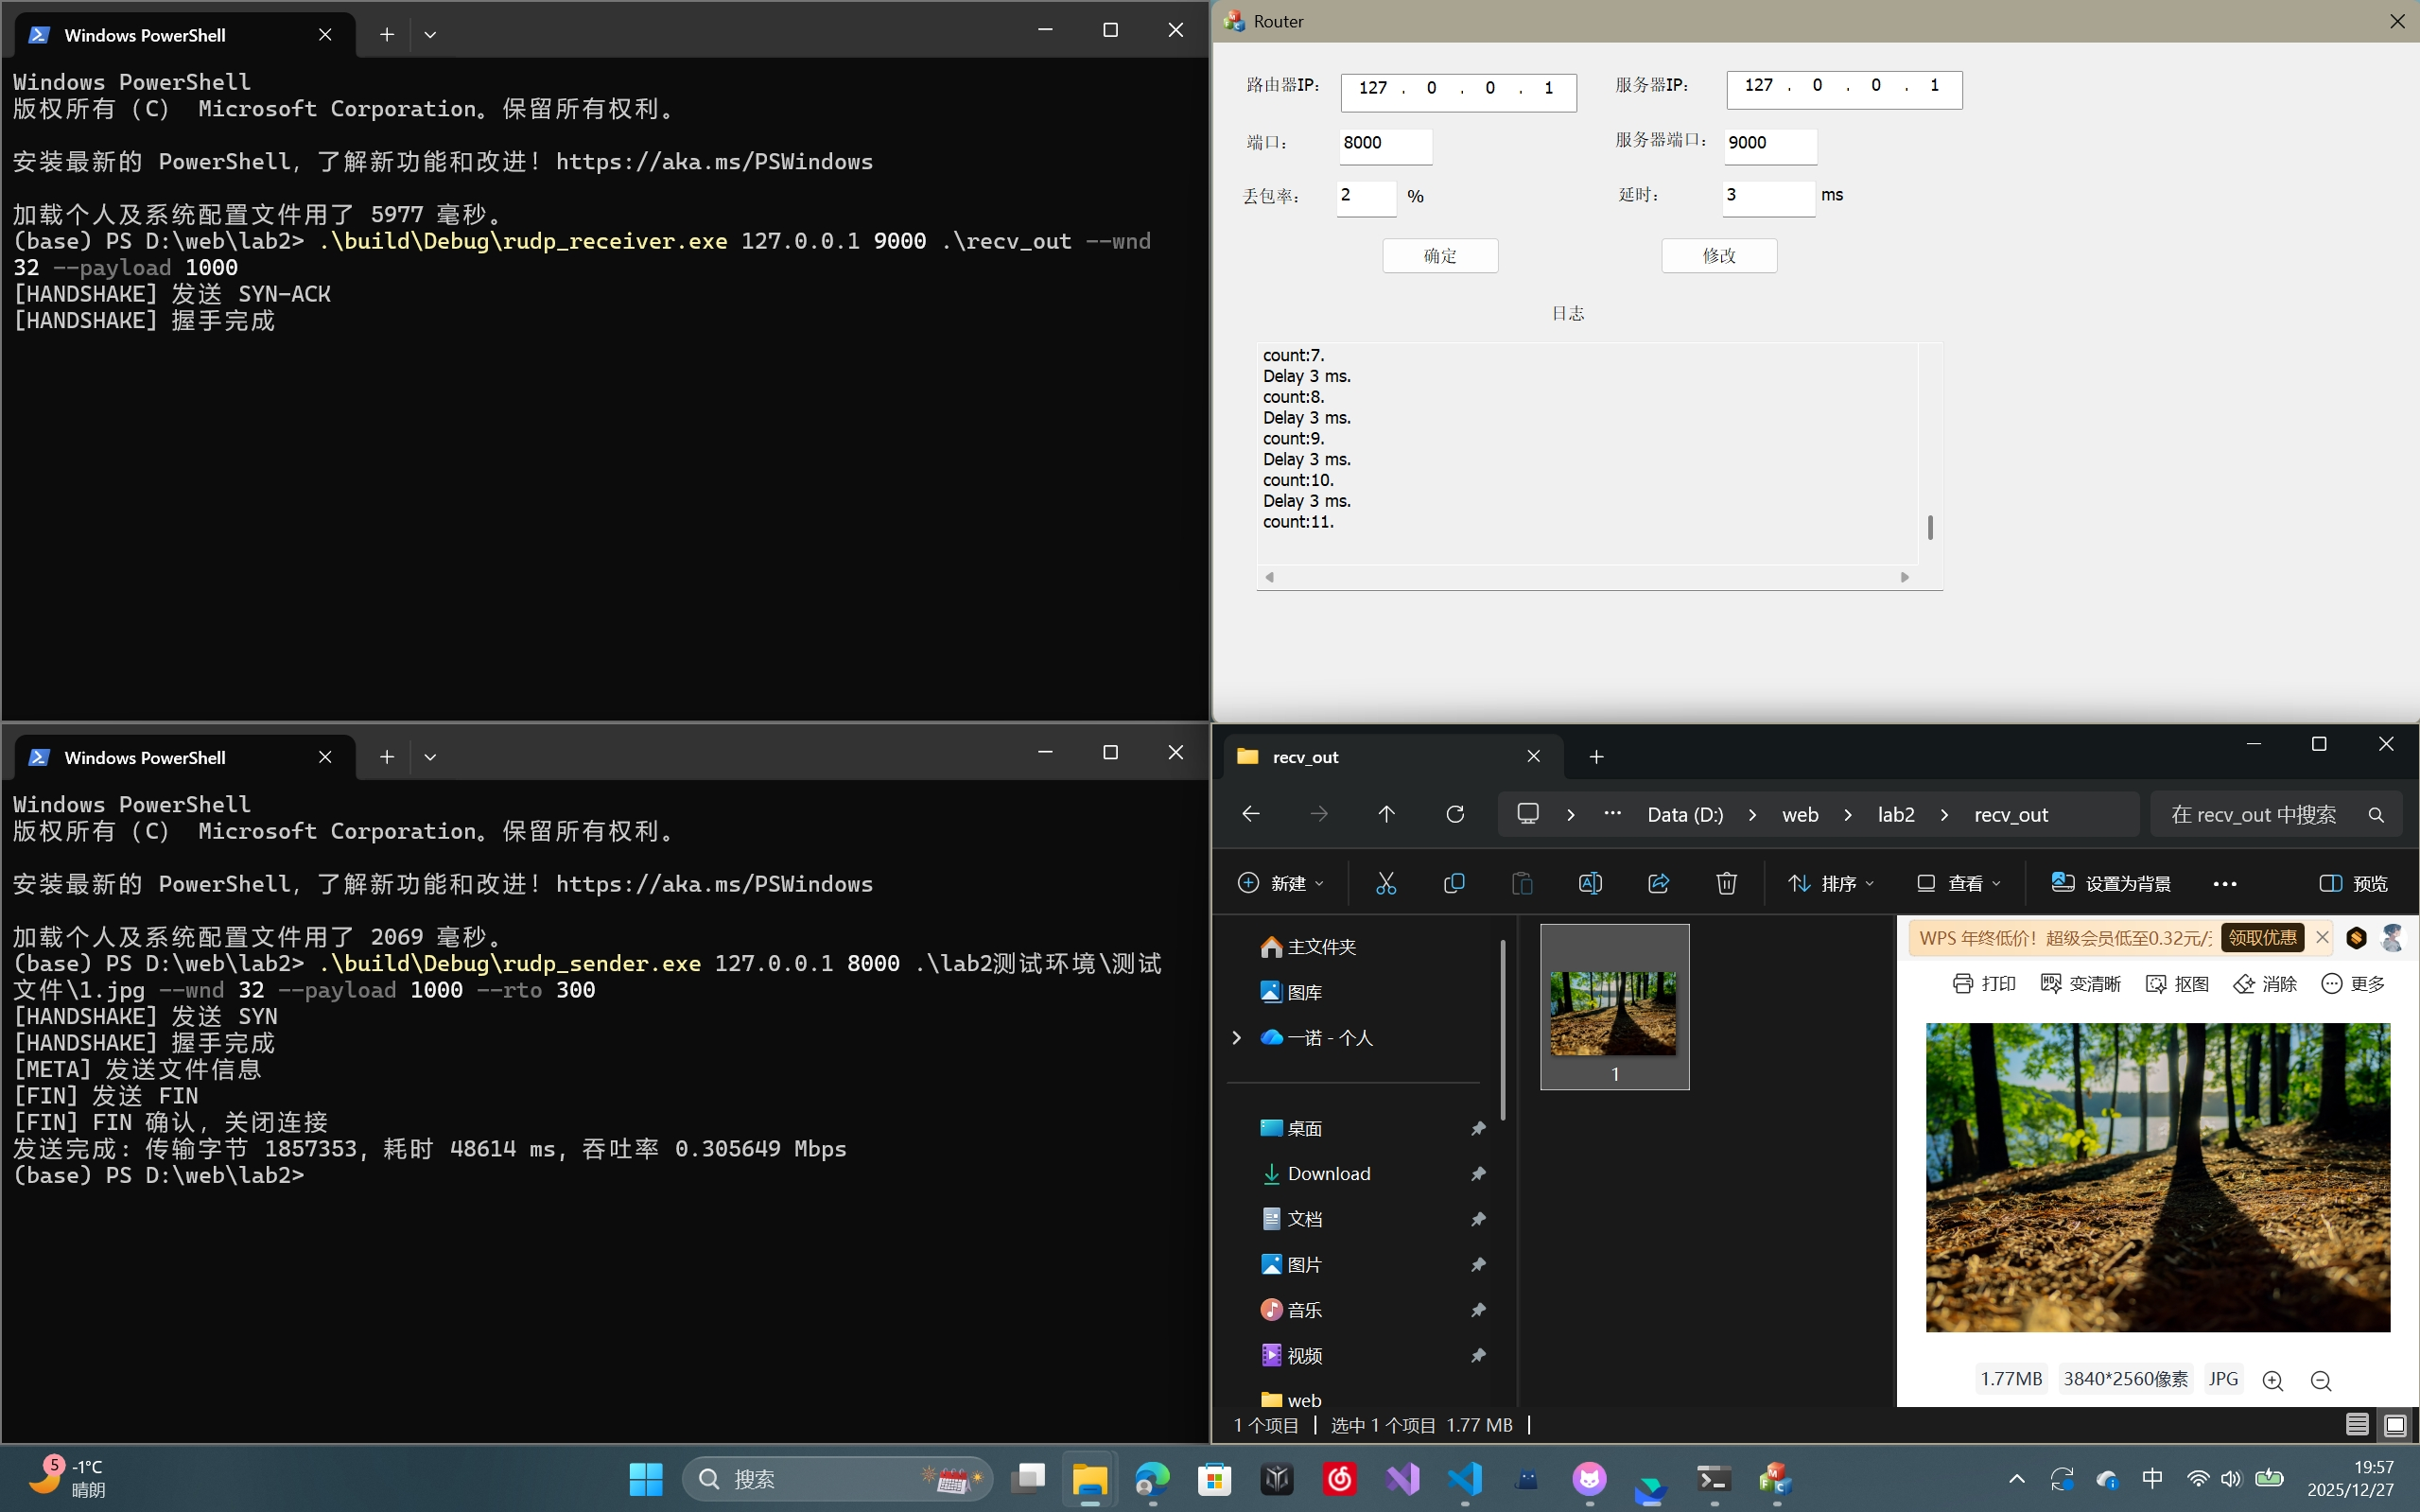
\includegraphics[width=\textwidth]{test.png}
		\caption{运行测试}
	\end{figure}

	可以看到双端成功通过Router传输了文件，图片文件也完整无误，且能看到在当前的丢包率和延时设置下，整体用时比直连要多了不少。
	
	\section{实验总结与改进方向}
	本次实验通过在用户空间实现基于 UDP 的可靠传输协议，深入理解了 TCP 协议栈的核心机制。成功实现了握手、确认、超时重传、SACK 选择重传、流量控制及 RENO 拥塞控制算法。
	
	\begin{itemize}
		\item \textbf{协议开销与效率}：通过引入 SACK 机制，显著减少了在丢包场景下的无效重传，相比于简单的 Go-Back-N 协议，大幅提升了带宽利用率。
		\item \textbf{拥塞控制的重要性}：实验观察到，如果没有拥塞控制，在网络状况波动时，固定速率发送极易导致丢包加剧，进而引发吞吐率雪崩。Reno 算法通过动态调整 cwnd，有效平衡了发送速率与网络容量。
		\item \textbf{可能的改进方向思考}：
		\begin{enumerate}
			\item \textbf{RTT 动态估算}：目前协议使用了固定的 RTO 超时重传时间。在实际广域网中，RTT 波动较大，可以实现动态计算 RTT 和 RTO，以更精准地判断超时。
			\item \textbf{更先进的拥塞控制}：可以尝试实现 TCP BBR 或其他算法，以在Long Fat Network中获得更好的性能。
			\item \textbf{双向数据传输}：当前实现仅支持单向文件传输，可扩展为全双工流式传输，以支持更复杂的应用场景。
		\end{enumerate}
	\end{itemize}
	
\end{document}
